\begin{frame}{The Landscape: Challenges of the Error Surface}
    \begin{itemize}
        \item The error surface for deep networks is complex and \bhighlight{non-convex}, presenting several challenges for gradient descent.
        \item \textbf{Local Minima:} These are points where the gradient is zero, but which are not the global minimum. While a concern, they are less of a problem in high-dimensional spaces than saddle points.
        \item \textbf{Saddle Points:} These are points where the gradient is also zero, but the function curves up in some directions and down in others. Gradient descent can get "stuck" and slow down significantly on them.
    \end{itemize}
    \begin{figure}
        \centering
        % Source: Optimization I.pdf, Page: 3
        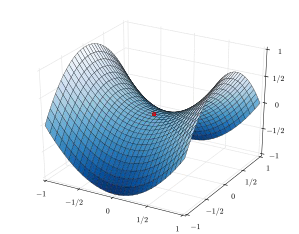
\includegraphics[width=0.4\linewidth]{images/saddle_point.png}
        \caption{A visualization of a saddle point.}
    \end{figure}
\end{frame}

\begin{frame}{The Landscape: Challenges of the Error Surface}
    \framesubtitle{Saddle Points vs. Local Minima}
    \begin{itemize}
        \item A popular and important hypothesis in deep learning is that in large networks, \bhighlight{saddle points are far more common} than local minima.
        \item For a point to be a local minimum, the curvature must be positive in \emph{all} dimensions. For a high-dimensional space, the probability of this is very low.
        \item Therefore, most points with zero gradient that our optimizer finds are likely to be saddle points, not "bad" local minima.
    \end{itemize}
    \begin{figure}
        \centering
        % Source: Optimization I.pdf, Page: 4
        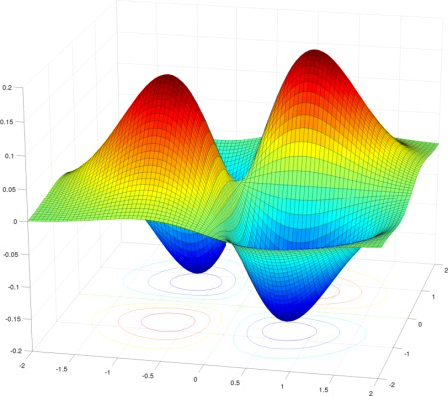
\includegraphics[width=0.5\linewidth]{images/error_surfaces.png}
        \caption{Examples of complex, non-convex error surfaces in neural networks.}
    \end{figure}
\end{frame}